\documentclass{article}
\usepackage{tikz}
\usetikzlibrary{shapes.geometric, arrows}
\tikzstyle{startstop} = [rectangle, rounded corners, minimum width=4cm, minimum height=1cm,text centered, draw=black, fill=red!30]
\tikzstyle{io} = [trapezium, trapezium left angle=70, trapezium right angle=110, minimum width=4cm, minimum height=1cm, text centered, draw=black, fill=blue!30]
\tikzstyle{process} = [rectangle, minimum width=3cm, minimum height=1cm, text centered, draw=black, fill=orange!30]
\tikzstyle{decision} = [diamond, minimum width=3cm, minimum height=1cm, text centered, draw=black, fill=green!30]
\tikzstyle{arrow} = [thick,->,>=stealth]


\begin{document}
% REGEX NER 
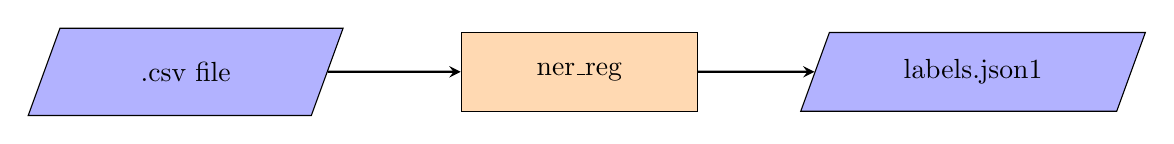
\begin{tikzpicture}[node distance=5cm]
\node (start) [io] {.csv file};
\node (module) [process, right of=start] {ner\_reg};
\node (stop) [io, right of=module] {labels.json1};
\draw [arrow] (start) -- (module);
\draw [arrow] (module) -- (stop);
\end{tikzpicture}
\newline
ner regex
\newline
\newline
\newline
% DATASET SPLITTER
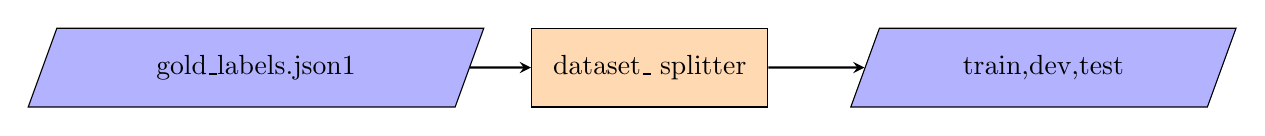
\begin{tikzpicture}[node distance=5cm]
\node (start) [io] {gold\_labels.json1};
\node (module) [process, right of=start] {dataset\_ splitter};
\node (stop) [io, right of=module] {train,dev,test};
\draw [arrow] (start) -- (module);
\draw [arrow] (module) -- (stop);
\end{tikzpicture}
\newline
dataset splitter
\newline
\newline
\newline
% SPACY NER 
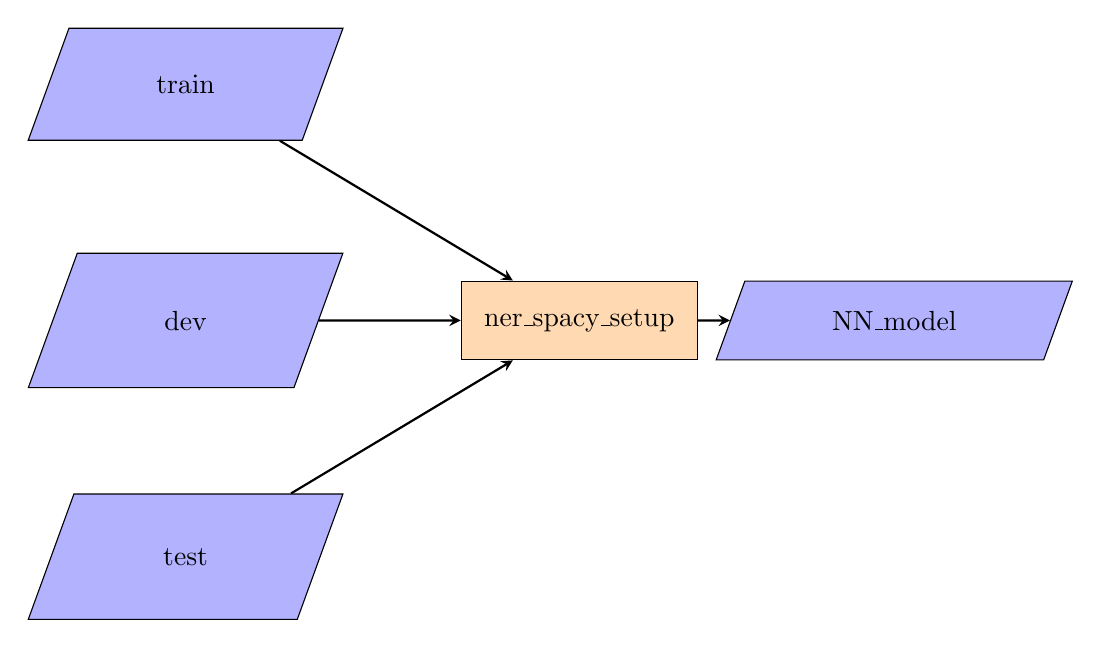
\begin{tikzpicture}[node distance=1cm]
\node (train) [io] {train};
\node (dev) [io, below of=train, node distance=3cm] {dev};
\node (test) [io, below of=dev, node distance=3cm] {test};
\node (module) [process, right of=dev, node distance=5cm] {ner\_spacy\_setup};
\node (stop) [io, right of=module, node distance=4cm] {NN\_model};
\draw [arrow] (train) -- (module);
\draw [arrow] (dev) -- (module);
\draw [arrow] (test) -- (module);
\draw [arrow] (module) -- (stop);
\end{tikzpicture}
\newline
ner spacy setup
\newline
\newline
\newline
% MODEL USAGE
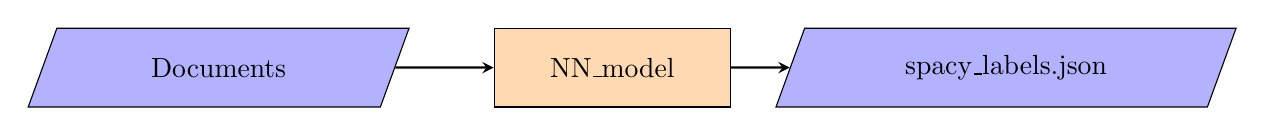
\begin{tikzpicture}[node distance=5cm]
\node (start) [io] {Documents};
\node (module) [process, right of=start] {NN\_model};
\node (stop) [io, right of=module] {spacy\_labels.json};
\draw [arrow] (start) -- (module);
\draw [arrow] (module) -- (stop);
\end{tikzpicture}
\newline
model usage
\newline
\newline
\newline
% SCORER
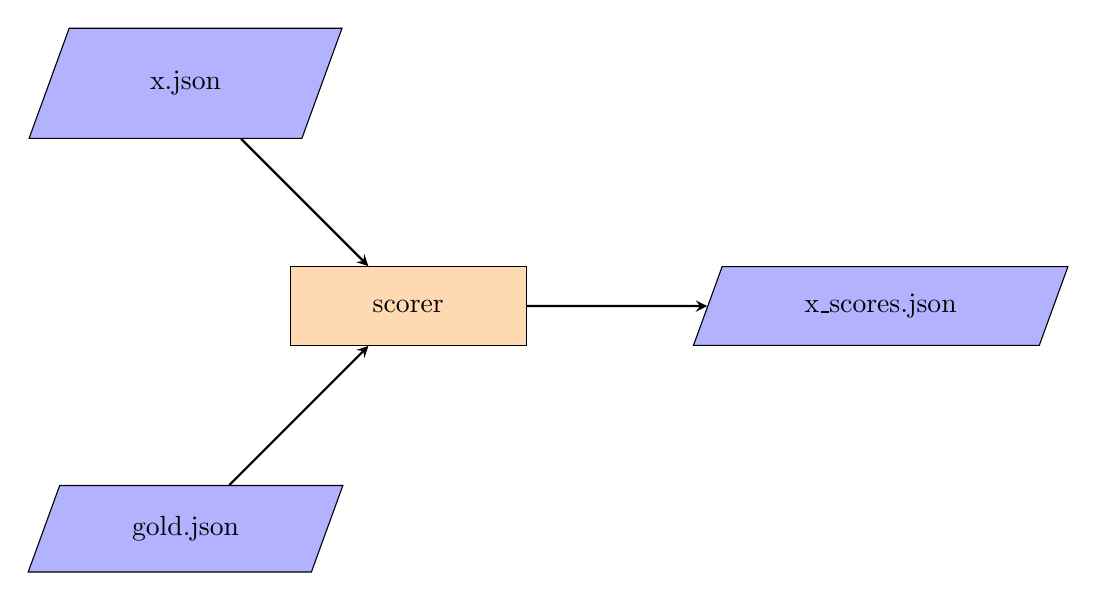
\begin{tikzpicture}[node distance=4cm]
\node (x) [io] {x.json};
\node (module) [process, below right of=x] {scorer};
\node (gold) [io, below left of=module] {gold.json};
\node (scores) [io, right of=module, node distance=6cm] {x\_scores.json};
\draw [arrow] (x) -- (module);
\draw [arrow] (gold) -- (module);
\draw [arrow] (module) -- (scores);
\end{tikzpicture}
\newline
scorer
\newline
\newline
\newline
% JSON TO CSV
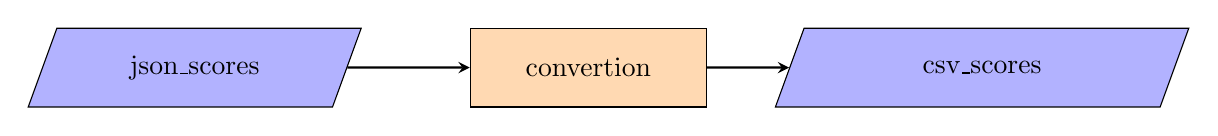
\begin{tikzpicture}[node distance=5cm]
\node (start) [io] {json\_scores}; %{Input};
\node (module) [process, right of=start] {convertion};
\node (stop) [io, right of=module] {csv\_scores}; %{Output};
\draw [arrow] (start) -- (module);
\draw [arrow] (module) -- (stop);
\end{tikzpicture}
\newline
conversion from json to csv


\end{document}
